\documentclass{beamer}\usepackage[]{graphicx}\usepackage[]{color}
%% maxwidth is the original width if it is less than linewidth
%% otherwise use linewidth (to make sure the graphics do not exceed the margin)
\makeatletter
\def\maxwidth{ %
  \ifdim\Gin@nat@width>\linewidth
    \linewidth
  \else
    \Gin@nat@width
  \fi
}
\makeatother

\definecolor{fgcolor}{rgb}{0.345, 0.345, 0.345}
\newcommand{\hlnum}[1]{\textcolor[rgb]{0.686,0.059,0.569}{#1}}%
\newcommand{\hlstr}[1]{\textcolor[rgb]{0.192,0.494,0.8}{#1}}%
\newcommand{\hlcom}[1]{\textcolor[rgb]{0.678,0.584,0.686}{\textit{#1}}}%
\newcommand{\hlopt}[1]{\textcolor[rgb]{0,0,0}{#1}}%
\newcommand{\hlstd}[1]{\textcolor[rgb]{0.345,0.345,0.345}{#1}}%
\newcommand{\hlkwa}[1]{\textcolor[rgb]{0.161,0.373,0.58}{\textbf{#1}}}%
\newcommand{\hlkwb}[1]{\textcolor[rgb]{0.69,0.353,0.396}{#1}}%
\newcommand{\hlkwc}[1]{\textcolor[rgb]{0.333,0.667,0.333}{#1}}%
\newcommand{\hlkwd}[1]{\textcolor[rgb]{0.737,0.353,0.396}{\textbf{#1}}}%
\let\hlipl\hlkwb

\usepackage{framed}
\makeatletter
\newenvironment{kframe}{%
 \def\at@end@of@kframe{}%
 \ifinner\ifhmode%
  \def\at@end@of@kframe{\end{minipage}}%
  \begin{minipage}{\columnwidth}%
 \fi\fi%
 \def\FrameCommand##1{\hskip\@totalleftmargin \hskip-\fboxsep
 \colorbox{shadecolor}{##1}\hskip-\fboxsep
     % There is no \\@totalrightmargin, so:
     \hskip-\linewidth \hskip-\@totalleftmargin \hskip\columnwidth}%
 \MakeFramed {\advance\hsize-\width
   \@totalleftmargin\z@ \linewidth\hsize
   \@setminipage}}%
 {\par\unskip\endMakeFramed%
 \at@end@of@kframe}
\makeatother

\definecolor{shadecolor}{rgb}{.97, .97, .97}
\definecolor{messagecolor}{rgb}{0, 0, 0}
\definecolor{warningcolor}{rgb}{1, 0, 1}
\definecolor{errorcolor}{rgb}{1, 0, 0}
\newenvironment{knitrout}{}{} % an empty environment to be redefined in TeX

\usepackage{alltt}
\usetheme{default}
%\usetheme{Malmoe}

\title[EC999: Quantitative Text Analysis]{EC999: Collocations} \def\newblock{\hskip .11em plus .33em minus .07em}


\def\Tiny{\fontsize{10pt}{10pt}\selectfont}
\def\smaller{\fontsize{8pt}{8pt}\selectfont}

\institute[Warwick]{University of Chicago \& University of Warwick}
\author[Thiemo Fetzer]{Thiemo Fetzer}

 \date{\today}

\usepackage{natbib}
\usepackage{amsmath}
\usepackage{hyperref}
\usepackage{graphicx}
\usepackage{graphics}

\usepackage{amsfonts}
\usepackage{amssymb}
\usepackage{pdfpages}
\usepackage{natbib}
\usepackage{hyperref}
%\usepackage{enumitem}
 \usepackage{pgffor}
\usepackage{booktabs,caption,fixltx2e}
\usepackage[flushleft]{threeparttable}
\usepackage{verbatim} 
\usepackage{cancel}
\newcommand\xxcancel[1]{\xcancel{#1}\vphantom{#1}}

\usepackage{mathtools,xparse}

\newenvironment{Description}
               {\list{}{\labelwidth=0pt \itemindent-\leftmargin
                        \let\makelabel\Descriptionlabel
                        % or whatever
               }}
               {\endlist}
\newcommand*\Descriptionlabel[1]{%
  \hspace\labelsep
  \normalfont%  reset current font setting
  \color{blue}\bfseries\sffamily% or whatever 
  #1}


\setbeamersize{text margin left = 16pt, text margin right = 16pt}
\newcommand{\code}[1]{\texttt{#1}}

\newenvironment<>{algorithm}[1][\undefined]{%
\begin{actionenv}#2%
\ifx#1\undefined%
   \def\insertblocktitle{Algorithm}%
\else%
   \def\insertblocktitle{Algorithm ({\em#1})}%
\fi%
\par%
\mode<presentation>{%
  \setbeamercolor{block title}{fg=white,bg=yellow!50!black}
  \setbeamercolor{block body}{fg=black,bg=yellow!20}
}%
\usebeamertemplate{block begin}\em}
{\par\usebeamertemplate{block end}\end{actionenv}}


\newenvironment<>{assumption}[1][\undefined]{%
\begin{actionenv}#2%
\ifx#1\undefined%
   \def\insertblocktitle{Assumption}%
\else%
   \def\insertblocktitle{Assumption ({\em#1})}%
\fi%
\par%
\mode<presentation>{%
  \setbeamercolor{block title}{fg=white,bg=blue!50!black}
  \setbeamercolor{block body}{fg=black,bg=blue!20}
}%
\usebeamertemplate{block begin}\em}
{\par\usebeamertemplate{block end}\end{actionenv}}

%changing spacing between knitr code and output
\usepackage{etoolbox} 
\makeatletter 
\preto{\@verbatim}{\topsep=0pt \partopsep=0pt } 
\makeatother
\renewenvironment{knitrout}{\setlength{\topsep}{0mm}}{}
\IfFileExists{upquote.sty}{\usepackage{upquote}}{}
\begin{document}



\AtBeginSection[]
{
 \begin{frame}<beamer>
 \frametitle{Plan}
 \tableofcontents[currentsection]
 \end{frame}
}
\maketitle
 

%%%%%%%%%%%%%%%%%%%%%%%%%%%%


%%%%%%%%%%%%%%%%%%%%%%%%%%%%%%%%%%%%%%%%%%%%%%%%%%%%%%%%%%
\begin{frame}{Collocations}

\begin{quote}\emph{Collocations} of a given word are statements of the habitual or customary places of that word.\end{quote}

\begin{itemize}
\item Noun phrases: ``strong tea'' and ``weapons of mass destruction''

\item Phrasal verbs: like ``to make up'', 

\item Stock phrases: ``the rich and powerful''
\end{itemize}

Collocations very useful for \emph{terminology extraction}.

\end{frame}
%%%%%%%%%%%%%%%%%%%%%%%%%%%%%%%%%%%%%%%%%%%%%%%%%%%%%%%%%%%%%%%%%%%%%%%%%


%%%%%%%%%%%%%%%%%%%%%%%%%%%%%%%%%%%%%%%%%%%%%%%%%%%%%%%%%%
\begin{frame}[fragile]{Measuring Political Slant}
\begin{figure}[h]
\begin{center}
\includegraphics[scale=.5]<1>{figures/genzkow-democrat.png}
\includegraphics[scale=.5]<2>{figures/genzkow-republican.png}
\end{center}
%\caption{\small{EU Enlargement in 2004}}
\end{figure}

Identify n-grams (\emph{collocations}) and extract those that are distinctively more likely to appear in the corpus of republican versus democratic congressional speeches.

Gentzkow, M., \& Shapiro, J. M. (2010). What Drives Media Slant? Evidence From U.S. Daily Newspapers. Econometrica, 78(1), 35–71.  

\end{frame}
%%%%%%%%%%%%%%%%%%%%%%%%%%%%%%%%%%%%%%%%%%%%%%%%%%%%%%%%%%%%%%%%%%%%%%%%%

\section{Heuristic Approaches}
%%%%%%%%%%%%%%%%%%%%%%%%%%%%%%%%%%%%%%%%%%%%%%%%%%%%%%%%%%
\begin{frame}[fragile]{A heuristic way of identifying collocations}
A simple heuristic approach to identify collocations is simply counting raw occurences of word sequences, e.g. $C(w_1, w_2)$
\begin{knitrout}\tiny
\definecolor{shadecolor}{rgb}{0.969, 0.969, 0.969}\color{fgcolor}\begin{kframe}
\begin{alltt}
\hlkwd{library}\hlstd{(quanteda)}
\hlkwd{library}\hlstd{(data.table)}
\hlkwd{data}\hlstd{(SOTUCorpus,} \hlkwc{package} \hlstd{=} \hlstr{"quantedaData"}\hlstd{)}
\hlstd{TOKENS} \hlkwb{<-} \hlkwd{unlist}\hlstd{(}\hlkwd{tokenize}\hlstd{(}\hlkwd{corpus_subset}\hlstd{(SOTUCorpus, Date} \hlopt{>} \hlstr{"1993-01-01"}\hlstd{),} \hlkwc{ngrams} \hlstd{=} \hlnum{2}\hlstd{,}
    \hlkwc{removeNumbers} \hlstd{=} \hlnum{TRUE}\hlstd{,} \hlkwc{removePunct} \hlstd{=} \hlnum{TRUE}\hlstd{,} \hlkwc{removeSymbols} \hlstd{=} \hlnum{TRUE}\hlstd{,} \hlkwc{concatenator} \hlstd{=} \hlstr{" "}\hlstd{))}
\hlstd{DF} \hlkwb{<-} \hlkwd{data.table}\hlstd{(}\hlkwc{token} \hlstd{= TOKENS,} \hlkwc{president} \hlstd{=} \hlkwd{names}\hlstd{(TOKENS))}
\hlstd{DF[, .N,} \hlkwc{by} \hlstd{= token][}\hlkwd{order}\hlstd{(N,} \hlkwc{decreasing} \hlstd{=} \hlnum{TRUE}\hlstd{)][}\hlnum{1}\hlopt{:}\hlnum{15}\hlstd{]}
\end{alltt}
\begin{verbatim}
##         token   N
##  1:    in the 603
##  2:    of the 577
##  3:    of our 386
##  4:    to the 324
##  5:    on the 271
##  6:   and the 264
##  7:   for the 250
##  8: the world 245
##  9:   we must 242
## 10:   we have 203
## 11:    we can 203
## 12:   we will 185
## 13:     to do 181
## 14: more than 170
## 15:    in our 167
\end{verbatim}
\end{kframe}
\end{knitrout}

selecting the most frequently occurring bigrams is not very interesting...

\end{frame}
%%%%%%%%%%%%%%%%%%%%%%%%%%%%%%%%%%%%%%%%%%%%%%%%%%%%%%%%%%%%%%%%%%%%%%%%%


%%%%%%%%%%%%%%%%%%%%%%%%%%%%%%%%%%%%%%%%%%%%%%%%%%%%%%%%%%
\begin{frame}[fragile]{A refinement to heuristic}
A simple method to make these more informative is to remove \emph{stopwords}. Quanteda has a nice feature facilitating this through the \code{removeFeatures()} function.

\begin{knitrout}\tiny
\definecolor{shadecolor}{rgb}{0.969, 0.969, 0.969}\color{fgcolor}\begin{kframe}
\begin{alltt}
\hlstd{TOKENS}\hlkwb{<-}\hlkwd{removeFeatures}\hlstd{(}\hlkwd{tokenize}\hlstd{(}\hlkwd{corpus_subset}\hlstd{(SOTUCorpus, Date}\hlopt{>}\hlstr{'1994-01-01'}\hlstd{),} \hlkwc{removePunct} \hlstd{=} \hlnum{TRUE}\hlstd{),}\hlkwd{stopwords}\hlstd{(}\hlstr{"english"}\hlstd{))}
\hlstd{TOKENS}\hlkwb{<-}\hlkwd{unlist}\hlstd{(}\hlkwd{tokens_ngrams}\hlstd{(TOKENS,} \hlkwc{n}\hlstd{=}\hlnum{2}\hlstd{,} \hlkwc{concatenator}\hlstd{=}\hlstr{" "}\hlstd{))}
\hlstd{DF}\hlkwb{<-}\hlkwd{data.table}\hlstd{(}\hlstr{"token"}\hlstd{=TOKENS,} \hlstr{"president"}\hlstd{=}\hlkwd{names}\hlstd{(TOKENS))}
\hlstd{DF}\hlkwb{<-}\hlstd{DF[, .N,} \hlkwc{by}\hlstd{=token][}\hlkwd{order}\hlstd{(N,} \hlkwc{decreasing}\hlstd{=}\hlnum{TRUE}\hlstd{)]}
\hlstd{DF}\hlopt{$}\hlstd{N}\hlkwb{<-}\hlkwd{as.numeric}\hlstd{(DF}\hlopt{$}\hlstd{N)}
\hlstd{DF[}\hlnum{1}\hlopt{:}\hlnum{10}\hlstd{]}
\end{alltt}
\begin{verbatim}
##               token   N
##  1:     health care 130
##  2: American people 117
##  3:   United States 106
##  4: Social Security  96
##  5:       men women  83
##  6:       make sure  73
##  7:    21st century  67
##  8:       years ago  59
##  9:       last year  53
## 10:    ask Congress  52
\end{verbatim}
\begin{alltt}
\hlcom{#DF<-DF[1:5000]}
\end{alltt}
\end{kframe}
\end{knitrout}

the resulting bigrams are much more intuitive. Though this still presents no formal statistical method.
\end{frame}
%%%%%%%%%%%%%%%%%%%%%%%%%%%%%%%%%%%%%%%%%%%%%%%%%%%%%%%%%%%%%%%%%%%%%%%%%


%%%%%%%%%%%%%%%%%%%%%%%%%%%%%%%%%%%%%%%%%%%%%%%%%%%%%%%%%%
\begin{frame}[fragile]{Another refinement to heuristic }
A further refinement due to Part of speech (POS) tag patterns for collocation filtering. We will talk more about POS, but here is just an illustration 
\begin{knitrout}\tiny
\definecolor{shadecolor}{rgb}{0.969, 0.969, 0.969}\color{fgcolor}\begin{kframe}
\begin{alltt}
\hlcom{# install.packages('pacman')}
\hlkwd{library}\hlstd{(pacman)}
\hlcom{# loads packages in development}
\hlstd{pacman}\hlopt{::}\hlkwd{p_load_gh}\hlstd{(}\hlkwd{c}\hlstd{(}\hlstr{"trinker/termco"}\hlstd{,} \hlstr{"trinker/tagger"}\hlstd{,} \hlstr{"trinker/textshape"}\hlstd{))}
\hlcom{# THIS TAKES A WHILE}
\hlstd{TAGGED} \hlkwb{<-} \hlkwd{unlist}\hlstd{(}\hlkwd{lapply}\hlstd{(}\hlkwd{lapply}\hlstd{(}\hlkwd{tag_pos}\hlstd{(DF}\hlopt{$}\hlstd{token), names),} \hlkwa{function}\hlstd{(}\hlkwc{x}\hlstd{)} \hlkwd{paste}\hlstd{(x,}
    \hlkwc{collapse} \hlstd{=} \hlstr{" "}\hlstd{)))}
\hlstd{DF} \hlkwb{<-} \hlkwd{cbind}\hlstd{(DF, TAGGED)}
\hlkwd{head}\hlstd{(DF)}
\end{alltt}
\begin{verbatim}
##              token   N   TAGGED
## 1:     health care 130    NN NN
## 2: American people 117   JJ NNS
## 3:   United States 106 NNP NNPS
## 4: Social Security  96  NNP NNP
## 5:       men women  83  NNS NNS
## 6:       make sure  73    VB JJ
\end{verbatim}
\end{kframe}
\end{knitrout}
We can now filter out individual sequences of words that are common.
\begin{knitrout}\tiny
\definecolor{shadecolor}{rgb}{0.969, 0.969, 0.969}\color{fgcolor}\begin{kframe}
\begin{verbatim}
##               token TAGGED        token TAGGED
## 1:      health care  NN NN 21st century  JJ NN
## 2: health insurance  NN NN    last year  JJ NN
## 3:      world power  NN NN    Last year  JJ NN
## 4:       tax relief  NN NN   first time  JJ NN
## 5:       tax credit  NN NN  high school  JJ NN
## 6:       child care  NN NN clean energy  JJ NN
\end{verbatim}
\end{kframe}
\end{knitrout}
\end{frame}
%%%%%%%%%%%%%%%%%%%%%%%%%%%%%%%%%%%%%%%%%%%%%%%%%%%%%%%%%%%%%%%%%%%%%%%%%


%%%%%%%%%%%%%%%%%%%%%%%%%%%%%%%%%%%%%%%%%%%%%%%%%%%%%%%%%%
\begin{frame}[fragile]{Word location distances}
An alternative method is to look at the distribution of distances between words in a corpus of texts and pick candidate word pairs as those that are ``nearby''.

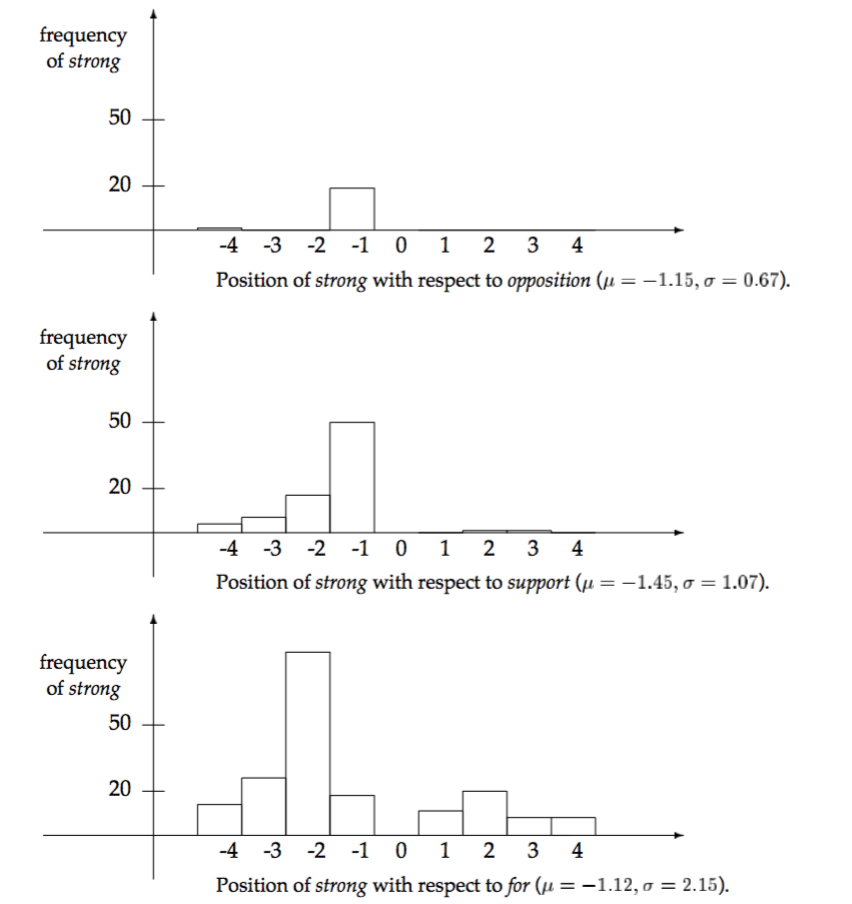
\includegraphics[scale=0.4]{figures/strong-opposition-example.png}

\end{frame}
%%%%%%%%%%%%%%%%%%%%%%%%%%%%%%%%%%%%%%%%%%%%%%%%%%%%%%%%%%%%%%%%%%%%%%%%%



%%%%%%%%%%%%%%%%%%%%%%%%%%%%%%%%%%%%%%%%%%%%%%%%%%%%%%%%%%
\begin{frame}{Summary Heuristic Approaches}
Can be surprisingly successful in identifying collocations. In this case, we saw that

\begin{enumerate}

\item A simple quantitative technique - a mere frequency filter 

\item Joint with the importance of parts of speech

\end{enumerate}

is able to produce quite some nice results.

We next turn to more formal statistical methods to identify and differentiate collocations.

\end{frame}
%%%%%%%%%%%%%%%%%%%%%%%%%%%%%%%%%%%%%%%%%%%%%%%%%%%%%%%%%%%%%%%%%%%%%%%%%



\section{Statistical Tests}
%%%%%%%%%%%%%%%%%%%%%%%%%%%%%%%%%%%%%%%%%%%%%%%%%%%%%%%%%%
\begin{frame}[fragile]{Formal Statistical Tests}
We now turn to formal statistical tests to identify collocations. The tests are all a variant of testing the hypothesis that the sequence of words is drawn at random, formally this hypothesis can be stated as

$$H_0: \quad P(w_1, w_2) = P(w_1) P(w_2)$$

We present three approaches

\begin{itemize}

\item Simple T-tests

\item $\chi^2$ tests (also used to evaluate similarity of corpora)

\item Likelihood ratio tests
\end{itemize}

\end{frame}
%%%%%%%%%%%%%%%%%%%%%%%%%%%%%%%%%%%%%%%%%%%%%%%%%%%%%%%%%%%%%%%%%%%%%%%%%


%%%%%%%%%%%%%%%%%%%%%%%%%%%%%%%%%%%%%%%%%%%%%%%%%%%%%%%%%%
\begin{frame}[fragile]{T-Tests}
For a word pair $w_1 w_2$, the hypothesis we want to test is whether:
$$H_0: P(w_1 w_2) = P(w_1) P(w_2)$$
We can estimate the three parameters by looking at our data and estimating the number of times a word appears. For example for the word pair \code{health care}.
\begin{knitrout}\tiny
\definecolor{shadecolor}{rgb}{0.969, 0.969, 0.969}\color{fgcolor}\begin{kframe}
\begin{alltt}
\hlstd{DF[token} \hlopt{==} \hlstr{"health care"}\hlstd{]}\hlopt{$}\hlstd{N}
\end{alltt}
\begin{verbatim}
## [1] 130
\end{verbatim}
\begin{alltt}
\hlkwd{sum}\hlstd{(DF[}\hlkwd{grep}\hlstd{(}\hlstr{"^\textbackslash{}\textbackslash{}bhealth\textbackslash{}\textbackslash{}b"}\hlstd{, token)]}\hlopt{$}\hlstd{N)}
\end{alltt}
\begin{verbatim}
## [1] 237
\end{verbatim}
\begin{alltt}
\hlkwd{sum}\hlstd{(DF[}\hlkwd{grep}\hlstd{(}\hlstr{"\textbackslash{}\textbackslash{}bcare\textbackslash{}\textbackslash{}b$"}\hlstd{, token)]}\hlopt{$}\hlstd{N)}
\end{alltt}
\begin{verbatim}
## [1] 239
\end{verbatim}
\begin{alltt}
\hlkwd{sum}\hlstd{(DF}\hlopt{$}\hlstd{N)}
\end{alltt}
\begin{verbatim}
## [1] 78631
\end{verbatim}
\end{kframe}
\end{knitrout}

Under the Null, this is a \emph{Bernoulli trial} whose probability of success we can estimate as:
\begin{eqnarray*}
P(\text{health care}) &=& P(\text{health}) \times P(\text{care})\\
&=& \frac{237}{\ensuremath{7.8631\times 10^{4}}} \times \frac{239}{\ensuremath{7.8631\times 10^{4}}} = \ensuremath{9.1613326\times 10^{-6}}
\end{eqnarray*}
\end{frame}
%%%%%%%%%%%%%%%%%%%%%%%%%%%%%%%%%%%%%%%%%%%%%%%%%%%%%%%%%%%%%%%%%%%%%%%%%


%%%%%%%%%%%%%%%%%%%%%%%%%%%%%%%%%%%%%%%%%%%%%%%%%%%%%%%%%%
\begin{frame}[fragile]{T-Tests}
\begin{knitrout}\tiny
\definecolor{shadecolor}{rgb}{0.969, 0.969, 0.969}\color{fgcolor}\begin{kframe}
\begin{alltt}
\hlstd{DF[token} \hlopt{==} \hlstr{"health care"}\hlstd{]}\hlopt{$}\hlstd{N}
\end{alltt}
\begin{verbatim}
## [1] 130
\end{verbatim}
\begin{alltt}
\hlkwd{sum}\hlstd{(DF}\hlopt{$}\hlstd{N)}
\end{alltt}
\begin{verbatim}
## [1] 78631
\end{verbatim}
\begin{alltt}
\hlstd{xbar} \hlkwb{=} \hlstd{DF[token} \hlopt{==} \hlstr{"health care"}\hlstd{]}\hlopt{$}\hlstd{N}\hlopt{/}\hlkwd{sum}\hlstd{(DF}\hlopt{$}\hlstd{N)}
\end{alltt}
\end{kframe}
\end{knitrout}
We estimate 
$$P(\text{health care}) =\frac{130}{\ensuremath{7.8631\times 10^{4}}}$$

Under $H_0$, T-statistic follows approximately a t-distribution with $N-1$ degrees of freedom.
$$T = \frac{\bar{x} - \mu}{\sqrt{\frac{s^2}{N}}}$$
with $\mu = $ and variance $\sigma^2 = p(1-p)$ (Variance of Bernoulli distribution).

So compute
$$T = \frac{0.0016533 - \ensuremath{9.1613326\times 10^{-6}}}{\sqrt{\frac{\ensuremath{9.1612486\times 10^{-6}}}{\ensuremath{7.8631\times 10^{4}}}}} = 152.3196326$$
\end{frame}
%%%%%%%%%%%%%%%%%%%%%%%%%%%%%%%%%%%%%%%%%%%%%%%%%%%%%%%%%%%%%%%%%%%%%%%%%

%%%%%%%%%%%%%%%%%%%%%%%%%%%%%%%%%%%%%%%%%%%%%%%%%%%%%%%%%%
\begin{frame}[fragile]{T-Tests for whole data frame}
\begin{knitrout}\tiny
\definecolor{shadecolor}{rgb}{0.969, 0.969, 0.969}\color{fgcolor}\begin{kframe}
\begin{alltt}
\hlstd{DF[,} \hlkwd{`:=`}\hlstd{(ttest, (N}\hlopt{/}\hlstd{total} \hlopt{-} \hlstd{c_1}\hlopt{/}\hlstd{total} \hlopt{*} \hlstd{c_2}\hlopt{/}\hlstd{total)}\hlopt{/}\hlstd{(((c_1}\hlopt{/}\hlstd{total} \hlopt{*} \hlstd{c_2}\hlopt{/}\hlstd{total} \hlopt{*}
    \hlstd{(}\hlnum{1} \hlopt{-} \hlstd{c_1}\hlopt{/}\hlstd{total} \hlopt{*} \hlstd{c_2}\hlopt{/}\hlstd{total))}\hlopt{/}\hlstd{total)}\hlopt{^}\hlnum{0.5}\hlstd{))]}
\hlstd{DF[}\hlkwd{order}\hlstd{(ttest,} \hlkwc{decreasing} \hlstd{=} \hlnum{TRUE}\hlstd{)][c_1} \hlopt{+} \hlstd{c_2} \hlopt{>} \hlnum{20}\hlstd{][}\hlnum{1}\hlopt{:}\hlnum{20}\hlstd{]}
\end{alltt}
\begin{verbatim}
##                    token   N   TAGGED total            w1          w2 c_1
##  1:   vacant storefronts  19   JJ NNS 78631        vacant storefronts  20
##  2:          Left Behind  11   VBN IN 78631          Left      Behind  11
##  3:      Social Security  96  NNP NNP 78631        Social    Security  96
##  4:           Child Left  11   NN VBN 78631         Child        Left  13
##  5:          Middle East  43  NNP NNP 78631        Middle        East  48
##  6:       Saddam Hussein  25  NNP NNP 78631        Saddam     Hussein  31
##  7:         Armed Forces  12 NNP NNPS 78631         Armed      Forces  12
##  8:        United States 106 NNP NNPS 78631        United      States 107
##  9:             al Qaeda  11   JJ NNP 78631            al       Qaeda  17
## 10:         minimum wage  24    NN NN 78631       minimum        wage  26
## 11:            men women  83  NNS NNS 78631           men       women 106
## 12:            God bless  28   NNP VB 78631           God       bless  47
## 13:         New Covenant  12  NNP NNP 78631           New    Covenant  23
## 14:      Tucson reminded  10  NNP VBD 78631        Tucson    reminded  14
## 15: distinguished guests  10  VBN NNS 78631 distinguished      guests  14
## 16:     mass destruction  17    NN NN 78631          mass destruction  24
## 17:      activist judges   8   NN NNS 78631      activist      judges   9
## 18:       teen pregnancy   7    JJ NN 78631          teen   pregnancy  13
## 19:       General ferret   7   NNP NN 78631       General      ferret  15
## 20:        Laden Zarqawi   7  NNP NNP 78631         Laden     Zarqawi  13
##     c_2    ttest
##  1:  19 273.2425
##  2:  12 268.4333
##  3: 108 264.0123
##  4:  11 257.8991
##  5:  46 256.4379
##  6:  25 251.7183
##  7:  16 242.7947
##  8: 141 241.5544
##  9:  11 225.5147
## 10:  36 219.8643
## 11: 115 210.4077
## 12:  30 208.9619
## 13:  12 202.4867
## 14:  14 200.2445
## 15:  14 200.2445
## 16:  25 194.5249
## 17:  15 193.0309
## 18:   8 192.4404
## 19:   7 191.5215
## 20:   9 181.4302
\end{verbatim}
\end{kframe}
\end{knitrout}
We condition on words occuring at least 20 times.
\end{frame}
%%%%%%%%%%%%%%%%%%%%%%%%%%%%%%%%%%%%%%%%%%%%%%%%%%%%%%%%%%%%%%%%%%%%%%%%%


%%%%%%%%%%%%%%%%%%%%%%%%%%%%%%%%%%%%%%%%%%%%%%%%%%%%%%%%%%
\begin{frame}[fragile]{T-Tests for whole data frame}
\begin{knitrout}\tiny
\definecolor{shadecolor}{rgb}{0.969, 0.969, 0.969}\color{fgcolor}\begin{kframe}
\begin{alltt}
\hlkwd{plot}\hlstd{(}\hlkwd{density}\hlstd{(DF}\hlopt{$}\hlstd{ttest),} \hlkwc{main} \hlstd{=} \hlstr{"Kernel Density of t-stats"}\hlstd{)}
\end{alltt}
\end{kframe}
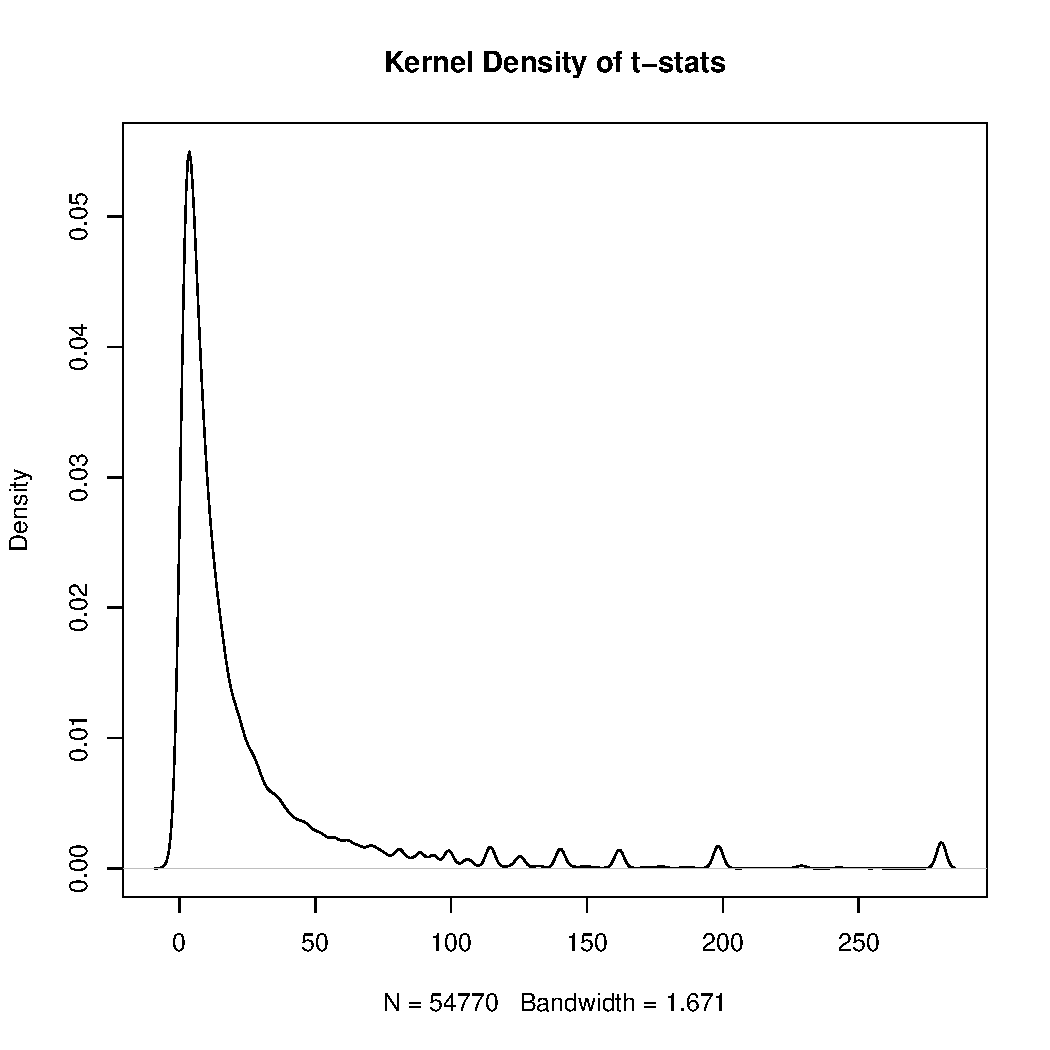
\includegraphics[width=3in]{figure/ttestexample4-1} 

\end{knitrout}
\end{frame}
%%%%%%%%%%%%%%%%%%%%%%%%%%%%%%%%%%%%%%%%%%%%%%%%%%%%%%%%%%%%%%%%%%%%%%%%%


%%%%%%%%%%%%%%%%%%%%%%%%%%%%%%%%%%%%%%%%%%%%%%%%%%%%%%%%%%
\begin{frame}[fragile]{Pearson's $\chi^2$ tests}
It turns out that t-tests are extremely optimistic (lots of false positives), but also that the underlying assumption of approximate normality is often invalid due to low counts. The $\chi^2$ test we discuss next is more useful and allows for meaningfull cross corpora analysis.
The $\chi^2$ test

\begin{itemize}

\item Compares the observed frequencies in the table with the frequencies expected for independence.

\item If the difference between observed and expected frequencies is large, then we can reject the null hypothesis of independence.
\end{itemize}
We can think of as word counts for a specific bigram to be arranged in tabular format
\begin{center}
  \begin{tabular}{ l | c | r }
    \hline
 & $w_1 = \text{health}$ &   $w_1 \neq \text{health}$ \\
$w_2 = \text{care}$ &  130 & 109 \\
$w_2 \neq \text{care}$ &  107 &  \ensuremath{7.8394\times 10^{4}} \\
    \hline
  \end{tabular}
\end{center}  
Note that $\sum_{j} C(w_1=\text{health},w_j) = C(w_1=\text{health})$.
\end{frame}
%%%%%%%%%%%%%%%%%%%%%%%%%%%%%%%%%%%%%%%%%%%%%%%%%%%%%%%%%%%%%%%%%%%%%%%%%



%%%%%%%%%%%%%%%%%%%%%%%%%%%%%%%%%%%%%%%%%%%%%%%%%%%%%%%%%%
\begin{frame}[fragile]{Pearson's $\chi^2$ tests}

We can think of as word counts for a specific bigram to be arranged in tabular format
\begin{center}
  \begin{tabular}{ l | c | r }
    \hline
 & $w_1 = \text{health}$ &   $w_1 \neq \text{health}$ \\
$w_2 = \text{care}$ &  130 & 109 \\
$w_2 \neq \text{care}$ &  107 &  \ensuremath{7.8394\times 10^{4}} \\
    \hline
  \end{tabular}
\end{center}  

The $\chi^2$ test statistic sums the differences between observed and expected values in all cells of the table, scaled by the magnitude of the expected values, as follows

$$X^2 = \sum_{ij}\frac{{(O_{ij} - E_{ij})^2}}{E_{ij}}$$

where $O_{ij}$ measures the observed count, while $E_{ij}$ measures the expected count. It is usually thought of as a measure of \emph{goodness of fit} to evaluate the fit of empirical against. $\chi^2$ tests are commonly implemented for collocation detected, e.g. in the \code{quanteda} R-package.
\end{frame}
%%%%%%%%%%%%%%%%%%%%%%%%%%%%%%%%%%%%%%%%%%%%%%%%%%%%%%%%%%%%%%%%%%%%%%%%%




%%%%%%%%%%%%%%%%%%%%%%%%%%%%%%%%%%%%%%%%%%%%%%%%%%%%%%%%%%
\begin{frame}[fragile]{Computing $\chi^2$ tests statistic}
\begin{center}
  \begin{tabular}{ l | c | c | c }
    \hline
 & $w_1 = \text{health}$ &   $w_1 \neq \text{health}$ &  \\
$w_2 = \text{care}$ &  130 & 109 & 239 \\
  &  0.7203647 & 238.2796353 &  \\
$w_2 \neq \text{care}$ &  107 & \ensuremath{7.8285\times 10^{4}} &  \ensuremath{7.8392\times 10^{4}} \\

  &  236.2796353 & \ensuremath{7.815572\times 10^{4}} &  \\
  
\hline
&  237 & \ensuremath{7.8394\times 10^{4}} &  \ensuremath{7.8631\times 10^{4}} \\
    \hline
  \end{tabular}
\end{center} 
\begin{itemize}
\item Expected frequencies $E_{ij}$ computed from the marginal probabilities; compute totals of rows and columns and  convert to proportions. 
\item Example: expected frequency (``health care'') is marginal probability of ``health'' occurring as the first part of a bigram times the marginal probability of ``care'' occurring as the second.
\end{itemize} 

\begin{eqnarray*}
X^2 = \frac{(130- 0.7203647)^2}{0.7203647} +  \frac{(109- 238.2796353)^2}{238.2796353}  \\
+ \frac{(107- 236.2796353)^2}{236.2796353} + \frac{(\ensuremath{7.8285\times 10^{4}}- \ensuremath{7.815572\times 10^{4}})^2}{{\ensuremath{7.815572\times 10^{4}}}}
\end{eqnarray*}




\end{frame}
%%%%%%%%%%%%%%%%%%%%%%%%%%%%%%%%%%%%%%%%%%%%%%%%%%%%%%%%%%%%%%%%%%%%%%%%%



%%%%%%%%%%%%%%%%%%%%%%%%%%%%%%%%%%%%%%%%%%%%%%%%%%%%%%%%%%
\begin{frame}[fragile]{Special formula for 2x2 tables}
\begin{center}
  \begin{tabular}{ l | c | c | c }
    \hline
 & $w_1 = \text{health}$ &   $w_1 \neq \text{health}$ &  \\
$w_2 = \text{care}$ &  130 & 109 & 239 \\
$w_2 \neq \text{care}$ &  107 & \ensuremath{7.8285\times 10^{4}} &  \ensuremath{7.8392\times 10^{4}} \\
\hline
&  237 & \ensuremath{7.8394\times 10^{4}} &  \ensuremath{7.8631\times 10^{4}} \\
    \hline
  \end{tabular}
\end{center} 

For 2 x 2 tables, there is a condensed formula [Can you show this?]
\begin{figure}[h]
\begin{center}
\includegraphics[scale=.6]<1>{figures/chi2-2x2.png}
\end{center}
%\caption{\small{EU Enlargement in 2004}}
\end{figure}

For a 2 x 2 design, this statistic has a $\chi^2$ distribution with one degree of freedom. Can you show that this statistic reaches maximal value in case off diagonals are zero (words exclusively appear together)?
\end{frame}
%%%%%%%%%%%%%%%%%%%%%%%%%%%%%%%%%%%%%%%%%%%%%%%%%%%%%%%%%%%%%%%%%%%%%%%%%



%%%%%%%%%%%%%%%%%%%%%%%%%%%%%%%%%%%%%%%%%%%%%%%%%%%%%%%%%%
\begin{frame}[fragile]{Identified Bigrams in State of the Union Speeches}
\begin{knitrout}\tiny
\definecolor{shadecolor}{rgb}{0.969, 0.969, 0.969}\color{fgcolor}\begin{kframe}
\begin{alltt}
\hlstd{DF[,} \hlkwd{`:=`}\hlstd{(O11, N)]}
\hlstd{DF[,} \hlkwd{`:=`}\hlstd{(O12, (c_2} \hlopt{-} \hlstd{N))]}
\hlstd{DF[,} \hlkwd{`:=`}\hlstd{(O21, (c_1} \hlopt{-} \hlstd{N))]}
\hlstd{DF[,} \hlkwd{`:=`}\hlstd{(O22, (total} \hlopt{-} \hlstd{c_1} \hlopt{-} \hlstd{c_2} \hlopt{+} \hlstd{N))]}
\hlstd{DF[,} \hlkwd{`:=`}\hlstd{(chi2, (total} \hlopt{*} \hlstd{(O11} \hlopt{*} \hlstd{O22} \hlopt{-} \hlstd{O12} \hlopt{*} \hlstd{O21)}\hlopt{^}\hlnum{2}\hlstd{)}\hlopt{/}\hlstd{((O11} \hlopt{+} \hlstd{O12)} \hlopt{*} \hlstd{(O11} \hlopt{+} \hlstd{O21)} \hlopt{*}
    \hlstd{(O12} \hlopt{+} \hlstd{O22)} \hlopt{*} \hlstd{(O21} \hlopt{+} \hlstd{O22)))]}

\hlstd{DF[c_1} \hlopt{+} \hlstd{c_2} \hlopt{>} \hlnum{20}\hlstd{][}\hlkwd{order}\hlstd{(chi2,} \hlkwc{decreasing} \hlstd{=} \hlnum{TRUE}\hlstd{)][}\hlnum{1}\hlopt{:}\hlnum{30}\hlstd{]}
\end{alltt}
\begin{verbatim}
##                    token   N   TAGGED total            w1          w2 c_1
##  1:   vacant storefronts  19   JJ NNS 78631        vacant storefronts  20
##  2:          Left Behind  11   VBN IN 78631          Left      Behind  11
##  3:      Social Security  96  NNP NNP 78631        Social    Security  96
##  4:           Child Left  11   NN VBN 78631         Child        Left  13
##  5:          Middle East  43  NNP NNP 78631        Middle        East  48
##  6:       Saddam Hussein  25  NNP NNP 78631        Saddam     Hussein  31
##  7:         Armed Forces  12 NNP NNPS 78631         Armed      Forces  12
##  8:        United States 106 NNP NNPS 78631        United      States 107
##  9:             al Qaeda  11   JJ NNP 78631            al       Qaeda  17
## 10:         minimum wage  24    NN NN 78631       minimum        wage  26
## 11:            men women  83  NNS NNS 78631           men       women 106
## 12:            God bless  28   NNP VB 78631           God       bless  47
## 13:         New Covenant  12  NNP NNP 78631           New    Covenant  23
## 14:      Tucson reminded  10  NNP VBD 78631        Tucson    reminded  14
## 15: distinguished guests  10  VBN NNS 78631 distinguished      guests  14
## 16:     mass destruction  17    NN NN 78631          mass destruction  24
## 17:      activist judges   8   NN NNS 78631      activist      judges   9
## 18:       teen pregnancy   7    JJ NN 78631          teen   pregnancy  13
## 19:       General ferret   7   NNP NN 78631       General      ferret  15
## 20:        Laden Zarqawi   7  NNP NNP 78631         Laden     Zarqawi  13
## 21:          White House  23  NNP NNP 78631         White       House  29
## 22:    preparing abandon  11   VBG NN 78631     preparing     abandon  15
## 23:          face bigger  49   NN RBR 78631          face      bigger 107
## 24:        playing field   9   VBG NN 78631       playing       field  15
## 25:        Madam Speaker  18  NNP NNP 78631         Madam     Speaker  18
## 26:          North Korea  12  NNP NNP 78631         North       Korea  25
## 27:       Vice President  43  NNP NNP 78631          Vice   President  46
## 28:           cold swept  10   NN VBN 78631          cold       swept  30
## 29:  chemical biological   9    NN JJ 78631      chemical  biological  19
## 30:        perfect Union  10   JJ NNP 78631       perfect       Union  11
##                    token   N   TAGGED total            w1          w2 c_1
##     c_2    ttest O11 O12 O21   O22     chi2
##  1:  19 273.2425  19   0   1 78611 74698.50
##  2:  12 268.4333  11   1   0 78619 72077.50
##  3: 108 264.0123  96  12   0 78523 69883.54
##  4:  11 257.8991  11   0   2 78618 66532.23
##  5:  46 256.4379  43   3   5 78580 65839.05
##  6:  25 251.7183  25   0   6 78600 63407.26
##  7:  16 242.7947  12   4   0 78615 58970.25
##  8: 141 241.5544 106  35   1 78489 58532.87
##  9:  11 225.5147  11   0   6 78614 50875.00
## 10:  36 219.8643  24  12   2 78593 48378.46
## 11: 115 210.4077  83  32  23 78493 44396.00
## 12:  30 208.9619  28   2  19 78582 43707.88
## 13:  12 202.4867  12   0  11 78608 41019.13
## 14:  14 200.2445  10   4   4 78613 40112.14
## 15:  14 200.2445  10   4   4 78613 40112.14
## 16:  25 194.5249  17   8   7 78599 37863.53
## 17:  15 193.0309   8   7   1 78615 37272.30
## 18:   8 192.4404   7   1   6 78617 37043.19
## 19:   7 191.5215   7   0   8 78616 36690.73
## 20:   9 181.4302   7   2   6 78616 32926.14
## 21:  44 180.4234  23  21   6 78581 32582.85
## 22:  21 173.7305  11  10   4 78606 30196.12
## 23:  62 168.4058  49  13  58 78511 28421.54
## 24:  15 168.1938   9   6   6 78610 28299.96
## 25:  51 166.4816  18  33   0 78580 27740.47
## 26:  17 163.1504  12   5  13 78601 26632.26
## 27: 120 162.0266  43  77   3 78508 26308.12
## 28:  10 161.8343  10   0  20 78601 26203.67
## 29:  13 160.5238   9   4  10 78608 25778.37
## 30:  29 156.9370  10  19   1 78601 24641.75
##     c_2    ttest O11 O12 O21   O22     chi2
\end{verbatim}
\end{kframe}
\end{knitrout}

\end{frame}
%%%%%%%%%%%%%%%%%%%%%%%%%%%%%%%%%%%%%%%%%%%%%%%%%%%%%%%%%%%%%%%%%%%%%%%%%


%%%%%%%%%%%%%%%%%%%%%%%%%%%%%%%%%%%%%%%%%%%%%%%%%%%%%%%%%%
\begin{frame}[fragile]{Identified Bigrams in State of the Union Speeches}
\begin{knitrout}\tiny
\definecolor{shadecolor}{rgb}{0.969, 0.969, 0.969}\color{fgcolor}\begin{kframe}
\begin{alltt}
\hlkwd{plot}\hlstd{(DF}\hlopt{$}\hlstd{ttest, DF}\hlopt{$}\hlstd{chi2)}
\end{alltt}
\end{kframe}
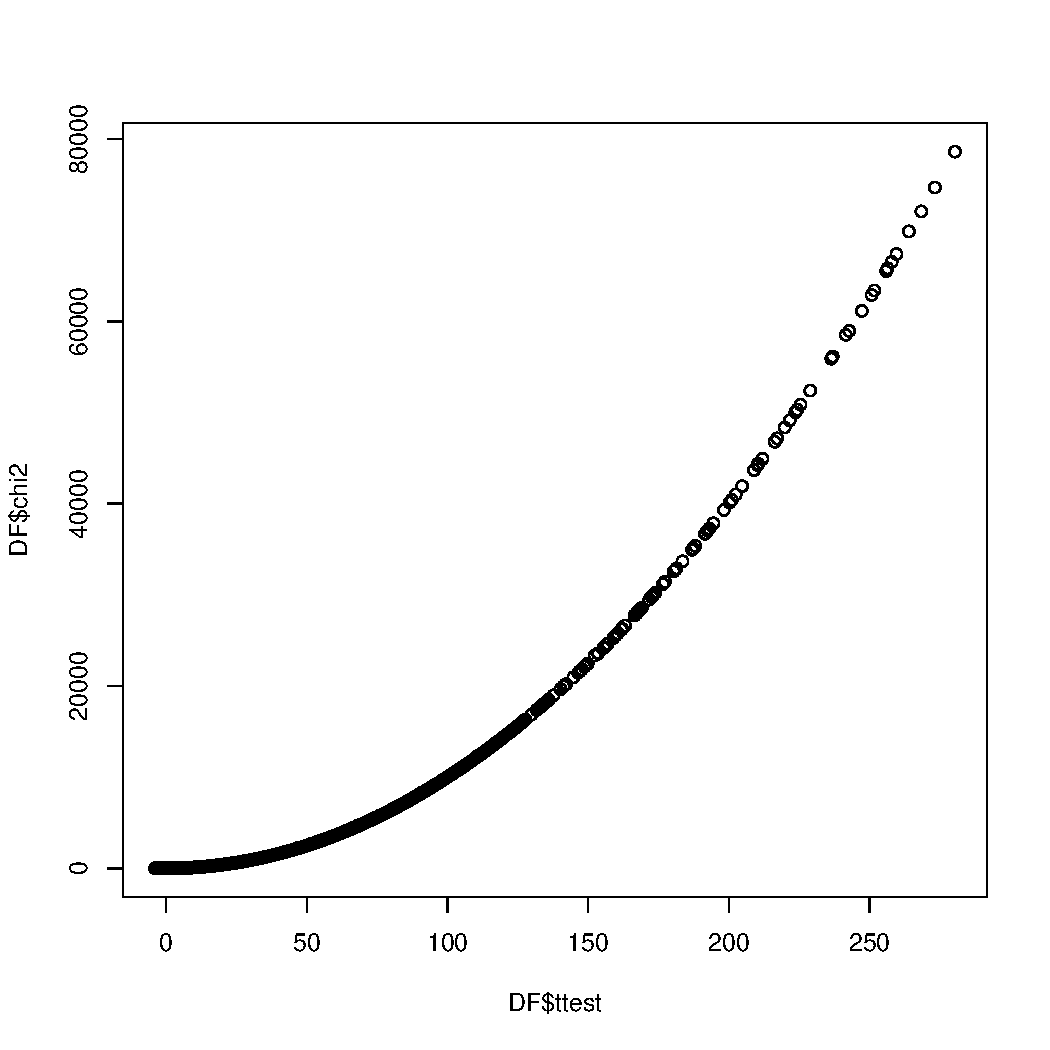
\includegraphics[width=3in]{figure/chisquareexample2-1} 

\end{knitrout}

\end{frame}
%%%%%%%%%%%%%%%%%%%%%%%%%%%%%%%%%%%%%%%%%%%%%%%%%%%%%%%%%%%%%%%%%%%%%%%%%


%%%%%%%%%%%%%%%%%%%%%%%%%%%%%%%%%%%%%%%%%%%%%%%%%%%%%%%%%%
\begin{frame}[fragile]{Problems for $\chi^2$ tests}

\begin{itemize}
\item T-test and $\chi^2$ test statistic provide almost identical ordering
\item $\chi^2$ test is also appropriate for large probabilities, for which the normality assumption of the t-test fails. 
\item But approximation to the chi-squared distribution breaks down if expected frequencies are too low. It will normally be acceptable so long as no more than 20\% of the events have expected frequencies below 5 (Read and Cressie 1988) $\rightarrow$ this is violated here.
\item Rule of thumb: advise against using $\chi^2$ if the expected value in any of the cells is 5 or less, use likelihood ratio test presented next.
\item In case of low expected counts, perform \emph{Yates correction}, modifying $X^2 = \sum_{ij}\frac{{|(O_{ij} - E_{ij}| -0.5)^2}}{E_{ij}}$

\end{itemize}

\end{frame}
%%%%%%%%%%%%%%%%%%%%%%%%%%%%%%%%%%%%%%%%%%%%%%%%%%%%%%%%%%%%%%%%%%%%%%%%%






%%%%%%%%%%%%%%%%%%%%%%%%%%%%%%%%%%%%%%%%%%%%%%%%%%%%%%%%%%
\begin{frame}[fragile]{Likelihood Ratio Tests}

Likelihood ratios are another approach to hypothesis testing. Developed in Dunning (1993), they are most appropriate for working with sparse data (few cell counts).

Two alternative hypothesis:
\begin{itemize}

\item Hypothesis 1: $P(w_2|w_1)  = p = P(w_2 | \neg w_1)$

\item Hypothesis 2: $P(w_2|w_1)  = p_1 \neq p_2 = P(w_2 | \neg w_1)$

\end{itemize}

Hypothesis is just another way of stating the independence assumption (a draw of word $w_2$ is independent of any information regarding the occurence or non-occurence of word $w_1$). Hypothesis 2  says that the probability of $w_2$ following $w_1$ is different from probability of $w_2$ not following $w_1$.\\

It is clear that $H_1$ is \emph{nested} into $H_2$.

\end{frame}
%%%%%%%%%%%%%%%%%%%%%%%%%%%%%%%%%%%%%%%%%%%%%%%%%%%%%%%%%%%%%%%%%%%%%%%%%


%%%%%%%%%%%%%%%%%%%%%%%%%%%%%%%%%%%%%%%%%%%%%%%%%%%%%%%%%%
\begin{frame}[fragile]{Likelihood ratio test}

Denote $c_1$, $c_2$ and $c_{12}$ , for the number of occurences of word $w_1$, $w_2$ and the pair $w_1 w_2$.
$$p = \frac{c_2}{N} \quad p_1 = \frac{c_{12}}{c_1} \quad p_2 = \frac{c_2 - c_{12}}{N- c_1}$$
We assume that word counts are binomially distributed
$$B(k; n,p) = \binom{n}{k} p^k (1-p)^{(n-k)}$$

Binomial distribution gives the probability of observing $k$ heads in a sequence of $n$ coin tosses, with success probability $p$.

What is the probability of observing counts $c_{12}$ in $c_1$ trials?
$$B(c_{12}; c_{1},p) = \binom{c_1}{c_{12}} p^{c_{12}} (1-p)^{(c_1-c_{12})}$$

What is the probability of observing counts $c_{2}-c_{12}$ in $N-c_{12}$ trials? I.e. probability of seeing $c_2$ by itself?

$$B(c_{2}-c_{12}; N-c_{12},p) = \binom{N-c_{12}}{c_{2}-c_{12}} p^{c_{2}-c_{12}} (1-p)^{(N-c_{12})}$$

\end{frame}
%%%%%%%%%%%%%%%%%%%%%%%%%%%%%%%%%%%%%%%%%%%%%%%%%%%%%%%%%%%%%%%%%%%%%%%%%


%%%%%%%%%%%%%%%%%%%%%%%%%%%%%%%%%%%%%%%%%%%%%%%%%%%%%%%%%%
\begin{frame}[fragile]{Likelihood ratio test}

Under Hypothesis 1 \& 2, the likelihood of observing counts are given as
\begin{eqnarray*}
L(H_1) = B(c_{12}; c_1,p)  B(c_2-c_{12}; N-c_1,p) \\
L(H_2) = B(c_{12}; c_1,p_1)  B(c_2-c_{12}; N-c_1,p_2)
\end{eqnarray*}
Likelihood ratio
\begin{eqnarray*}
\log(\lambda) &=& \log{\frac{L(H_1)}{L(H_2)}} \\
  & = & \log( p^{(c_1-c_{12})} (1-p)^{c_1}) + \log(p^{(c_2-c_{12})} (1-p)^{(N-c_1)}) \\
  & & - \log( p_1^{(c_1-c_{12})} (1-p_1)^{c_1}) - \log(p_2^{(c_2-c_{12})} (1-p_2)^{(N-c_1)})
\end{eqnarray*}
\end{frame}
%%%%%%%%%%%%%%%%%%%%%%%%%%%%%%%%%%%%%%%%%%%%%%%%%%%%%%%%%%%%%%%%%%%%%%%%%



%%%%%%%%%%%%%%%%%%%%%%%%%%%%%%%%%%%%%%%%%%%%%%%%%%%%%%%%%%
\begin{frame}[fragile]{Advantage of LR test}

\begin{itemize}

\item One advantage of likelihood ratios is that they have a clear intuitive interpretation: the $\exp$ of the LR provides a number that tells us how much more likely one hypothesis is than the other.

\item So numbers are easier to interpret than the scores of the $\chi^2$  test 

\item If $\lambda$  is a likelihood ratio of a particular form, then the quantity $-2 \log{\lambda}$ is asymptotically $\chi^2$ distributed 

\item Dunning (1993) shows they are more appropriate for sparse data.



\end{itemize}


\end{frame}
%%%%%%%%%%%%%%%%%%%%%%%%%%%%%%%%%%%%%%%%%%%%%%%%%%%%%%%%%%%%%%%%%%%%%%%%%





\section{Application: $\chi^2$ test for corpus similarity}



%%%%%%%%%%%%%%%%%%%%%%%%%%%%%%%%%%%%%%%%%%%%%%%%%%%%%%%%%%
\begin{frame}[fragile]{$\chi^2$ test for corpus similarity}

\begin{itemize}

\item So far, we have used various statistical tests to study whether words appearing together appear so in a non-random fashion.

\item We were comparing observed frequencies of pairs appearing with some notion of expected frequency under a null-hypothesis of independence.

\item We can apply the same test to distinguish word use \emph{between} texts.

\item The null-hypothesis here is that the probability of observing a word or a word pair is independent across speakers.

\end{itemize}
\end{frame}
%%%%%%%%%%%%%%%%%%%%%%%%%%%%%%%%%%%%%%%%%%%%%%%%%%%%%%%%%%%%%%%%%%%%%%%%%



%%%%%%%%%%%%%%%%%%%%%%%%%%%%%%%%%%%%%%%%%%%%%%%%%%%%%%%%%%
\begin{frame}[fragile]{$\chi^2$ test for corpus similarity}
We can use the $\chi^2$ statistic to differentiate two corpora from one another or to identify distinctive word features characteristic of a corpus. Below is an example of Bush versus Obama state of the union speeches.
\begin{knitrout}\tiny
\definecolor{shadecolor}{rgb}{0.969, 0.969, 0.969}\color{fgcolor}\begin{kframe}
\begin{alltt}
\hlstd{TOK} \hlkwb{<-} \hlkwd{data.table}\hlstd{(}\hlkwc{sotu} \hlstd{=} \hlkwd{names}\hlstd{(TOKENS),} \hlkwc{token} \hlstd{= TOKENS)}
\hlstd{TOK[,} \hlkwd{`:=`}\hlstd{(president,} \hlkwd{str_extract}\hlstd{(sotu,} \hlstr{"([A-z]*)"}\hlstd{))]}
\hlstd{TOK} \hlkwb{<-} \hlstd{TOK[, .N,} \hlkwc{by} \hlstd{=} \hlkwd{c}\hlstd{(}\hlstr{"president"}\hlstd{,} \hlstr{"token"}\hlstd{)][president} \hlopt \hlkwd{c}\hlstd{(}\hlstr{"Bush"}\hlstd{,} \hlstr{"Obama"}\hlstd{)]}
\hlstd{TOK[}\hlkwd{order}\hlstd{(N,} \hlkwc{decreasing} \hlstd{=} \hlnum{TRUE}\hlstd{)][}\hlnum{1}\hlopt{:}\hlnum{20}\hlstd{]}
\end{alltt}
\begin{verbatim}
##     president            token  N
##  1:      Bush  Social Security 45
##  2:      Bush    United States 44
##  3:     Obama      health care 44
##  4:     Obama  American people 44
##  5:      Bush        men women 41
##  6:     Obama    United States 37
##  7:      Bush      health care 34
##  8:      Bush    ground United 33
##  9:     Obama        make sure 31
## 10:     Obama      face bigger 28
## 11:     Obama     clean energy 28
## 12:     Obama        right now 27
## 13:      Bush  American people 26
## 14:      Bush      Middle East 26
## 15:      Bush     America will 25
## 16:     Obama        years ago 24
## 17:      Bush Members Congress 23
## 18:     Obama   States America 23
## 19:      Bush   Saddam Hussein 22
## 20:      Bush       tax relief 21
\end{verbatim}
\end{kframe}
\end{knitrout}
\end{frame}
%%%%%%%%%%%%%%%%%%%%%%%%%%%%%%%%%%%%%%%%%%%%%%%%%%%%%%%%%%%%%%%%%%%%%%%%%


%%%%%%%%%%%%%%%%%%%%%%%%%%%%%%%%%%%%%%%%%%%%%%%%%%%%%%%%%%
\begin{frame}[fragile]{$\chi^2$ test to identify distinct words across corpora}

We can coonvert this into wide format and compute the $\chi^2$ test statistic for each word feature, i.e. computing

\begin{figure}[h]
\begin{center}
\includegraphics[scale=.6]<1>{figures/chi2-2x2.png}
\end{center}
%\caption{\small{EU Enlargement in 2004}}
\end{figure}

\begin{knitrout}\tiny
\definecolor{shadecolor}{rgb}{0.969, 0.969, 0.969}\color{fgcolor}\begin{kframe}
\begin{alltt}
\hlstd{WIDE} \hlkwb{<-} \hlkwd{data.table}\hlstd{(}\hlkwd{join}\hlstd{(TOK[president} \hlopt{==} \hlstr{"Bush"}\hlstd{][,} \hlkwd{list}\hlstd{(token,} \hlkwc{bushcount} \hlstd{=} \hlkwd{as.numeric}\hlstd{(N))],}
    \hlstd{TOK[president} \hlopt{==} \hlstr{"Obama"}\hlstd{][,} \hlkwd{list}\hlstd{(token,} \hlkwc{obamacount} \hlstd{=} \hlkwd{as.numeric}\hlstd{(N))],} \hlkwc{type} \hlstd{=} \hlstr{"full"}\hlstd{))}
\hlstd{WIDE[}\hlkwd{is.na}\hlstd{(obamacount)]}\hlopt{$}\hlstd{obamacount} \hlkwb{<-} \hlnum{0}
\hlstd{WIDE[}\hlkwd{is.na}\hlstd{(bushcount)]}\hlopt{$}\hlstd{bushcount} \hlkwb{<-} \hlnum{0}
\hlstd{WIDE[,} \hlkwd{`:=`}\hlstd{(totalcount, obamacount} \hlopt{+} \hlstd{bushcount)]}
\hlstd{WIDE} \hlkwb{<-} \hlstd{WIDE[}\hlkwd{order}\hlstd{(totalcount,} \hlkwc{decreasing} \hlstd{=} \hlnum{TRUE}\hlstd{)][totalcount} \hlopt{>} \hlnum{5}\hlstd{]}
\hlstd{WIDE[,} \hlkwd{`:=`}\hlstd{(totalobama,} \hlkwd{sum}\hlstd{(obamacount))]}
\hlstd{WIDE[,} \hlkwd{`:=`}\hlstd{(totalbush,} \hlkwd{sum}\hlstd{(bushcount))]}
\hlstd{WIDE[,} \hlkwd{`:=`}\hlstd{(chi2, (totalobama} \hlopt{+} \hlstd{totalbush)} \hlopt{*} \hlstd{(bushcount} \hlopt{*} \hlstd{(totalobama} \hlopt{-} \hlstd{obamacount)} \hlopt{-}
    \hlstd{obamacount} \hlopt{*} \hlstd{(totalbush} \hlopt{-} \hlstd{bushcount))}\hlopt{^}\hlnum{2}\hlopt{/}\hlstd{((bushcount} \hlopt{+} \hlstd{obamacount)} \hlopt{*} \hlstd{(bushcount} \hlopt{+}
    \hlstd{(totalbush} \hlopt{-} \hlstd{bushcount))} \hlopt{*} \hlstd{(obamacount} \hlopt{+} \hlstd{(totalobama} \hlopt{-} \hlstd{obamacount))} \hlopt{*} \hlstd{((totalbush} \hlopt{-}
    \hlstd{bushcount)} \hlopt{+} \hlstd{(totalobama} \hlopt{-} \hlstd{obamacount))))]}
\end{alltt}
\end{kframe}
\end{knitrout}
\end{frame}
%%%%%%%%%%%%%%%%%%%%%%%%%%%%%%%%%%%%%%%%%%%%%%%%%%%%%%%%%%%%%%%%%%%%%%%%%

%%%%%%%%%%%%%%%%%%%%%%%%%%%%%%%%%%%%%%%%%%%%%%%%%%%%%%%%%%
\begin{frame}[fragile]{$\chi^2$ test to identify distinct words across corpora}
Present list sorted by $X^2$ test statistic score
\begin{knitrout}\tiny
\definecolor{shadecolor}{rgb}{0.969, 0.969, 0.969}\color{fgcolor}\begin{kframe}
\begin{alltt}
\hlstd{WIDE[}\hlnum{1}\hlopt{:}\hlnum{20}\hlstd{][}\hlkwd{order}\hlstd{(chi2,} \hlkwc{decreasing} \hlstd{=} \hlnum{TRUE}\hlstd{)]}
\end{alltt}
\begin{verbatim}
##                token bushcount obamacount totalcount totalobama totalbush
##  1:  Social Security        45         11         56       2225      1776
##  2:    ground United        33          5         38       2225      1776
##  3:        right now         1         27         28       2225      1776
##  4:     clean energy         2         28         30       2225      1776
##  5: Members Congress        23          5         28       2225      1776
##  6:      Middle East        26          7         33       2225      1776
##  7:        men women        41         21         62       2225      1776
##  8:      face bigger         8         28         36       2225      1776
##  9:     America will        25         14         39       2225      1776
## 10:   States America         7         23         30       2225      1776
## 11:        years ago         8         24         32       2225      1776
## 12:   every American         7         21         28       2225      1776
## 13:     ask Congress        18         11         29       2225      1776
## 14:    United States        44         37         81       2225      1776
## 15:        will help        16         10         26       2225      1776
## 16:        make sure        16         31         47       2225      1776
## 17: health insurance        16         12         28       2225      1776
## 18:  American people        26         44         70       2225      1776
## 19:    will continue        18         16         34       2225      1776
## 20:      health care        34         44         78       2225      1776
##            chi2
##  1: 29.76542402
##  2: 28.01000046
##  3: 19.03112218
##  4: 17.42404175
##  5: 16.28159834
##  6: 15.95019450
##  7: 12.05764904
##  8:  7.23091592
##  9:  6.20036699
## 10:  5.42860232
## 11:  4.91256175
## 12:  4.29416383
## 13:  3.69904010
## 14:  3.30379030
## 15:  3.11799054
## 16:  2.06237752
## 17:  1.85806910
## 18:  1.51540879
## 19:  1.01604414
## 20:  0.02058143
\end{verbatim}
\end{kframe}
\end{knitrout}
We had already removed stopwords, but we can exctract distinct part of speech pairs common for
\end{frame}
%%%%%%%%%%%%%%%%%%%%%%%%%%%%%%%%%%%%%%%%%%%%%%%%%%%%%%%%%%%%%%%%%%%%%%%%%

%%%%%%%%%%%%%%%%%%%%%%%%%%%%%%%%%%%%%%%%%%%%%%%%%%%%%%%%%%
\begin{frame}[fragile]{Combine this with POS Tag patterns}
\begin{knitrout}\tiny
\definecolor{shadecolor}{rgb}{0.969, 0.969, 0.969}\color{fgcolor}\begin{kframe}
\begin{alltt}
\hlstd{WIDE} \hlkwb{<-} \hlkwd{join}\hlstd{(WIDE, DF[,} \hlkwd{list}\hlstd{(token, TAGGED)])[}\hlkwd{grep}\hlstd{(}\hlstr{"NN.? NN.?|JJ.? NN.?"}\hlstd{, TAGGED)]}
\hlstd{WIDE[}\hlnum{1}\hlopt{:}\hlnum{20}\hlstd{][}\hlkwd{order}\hlstd{(chi2,} \hlkwc{decreasing} \hlstd{=} \hlnum{TRUE}\hlstd{)]}
\end{alltt}
\begin{verbatim}
##                token bushcount obamacount totalcount totalobama totalbush
##  1:  Social Security        45         11         56       2225      1776
##  2:    ground United        33          5         38       2225      1776
##  3:   Saddam Hussein        22          0         22       2225      1776
##  4:       tax relief        21          2         23       2225      1776
##  5:     clean energy         2         28         30       2225      1776
##  6: Members Congress        23          5         28       2225      1776
##  7:      Middle East        26          7         33       2225      1776
##  8:  fellow citizens        20          4         24       2225      1776
##  9:        men women        41         21         62       2225      1776
## 10:       first time         2         20         22       2225      1776
## 11:        hard work         3         15         18       2225      1776
## 12:   States America         7         23         30       2225      1776
## 13:    United States        44         37         81       2225      1776
## 14:      high school         7         19         26       2225      1776
## 15:        last year         7         17         24       2225      1776
## 16: health insurance        16         12         28       2225      1776
## 17:  American people        26         44         70       2225      1776
## 18: small businesses        10         14         24       2225      1776
## 19:      health care        34         44         78       2225      1776
## 20:   Vice President        10         12         22       2225      1776
##            chi2   TAGGED
##  1: 29.76542402  NNP NNP
##  2: 28.01000046   NN NNP
##  3: 27.71432764  NNP NNP
##  4: 20.62658903    NN NN
##  5: 17.42404175    JJ NN
##  6: 16.28159834  NNS NNP
##  7: 15.95019450  NNP NNP
##  8: 14.83470943   NN NNS
##  9: 12.05764904  NNS NNS
## 10: 11.16558446    JJ NN
## 11:  5.62926109    JJ NN
## 12:  5.42860232  NNP NNP
## 13:  3.30379030 NNP NNPS
## 14:  3.23405308    JJ NN
## 15:  2.26644527    JJ NN
## 16:  1.85806910    NN NN
## 17:  1.51540879   JJ NNS
## 18:  0.07248363   JJ NNS
## 19:  0.02058143    NN NN
## 20:  0.01017665  NNP NNP
\end{verbatim}
\end{kframe}
\end{knitrout}
\end{frame}
%%%%%%%%%%%%%%%%%%%%%%%%%%%%%%%%%%%%%%%%%%%%%%%%%%%%%%%%%%%%%%%%%%%%%%%%%




\end{document}

